\documentclass{report}
\usepackage[acronym,automake]{glossaries-extra}
\usepackage{hyperref}
\usepackage{unicode}
\usepackage{apacite}
\usepackage{parskip}
\usepackage{graphicx}
\usepackage{tabularx}
\usepackage{lipsum}
\setabbreviationstyle[acronym]{long-short}
\newacronym{startup}{fotogramas de inicio}{Cantidad de fotogramas para comenzar una movida}
\newacronym{active}{fotogramas activos}{Cantidad de fotogramas en la cual es posible colisionar con el oponente}
\newacronym{recovery}{fotogramas de recuperación}{Cantidad de fotogramas en la cual es imposible admitir otra movida}
\newacronym{frame_data}{datos fotográmicos}{los valores de fotogramas de inicio, fotogramas activos, fotogramas de recuperación y aturdimiento de bloqueo para una movida}
\newacronym{on_block}{bloqueando}{Cantidad de fotogramas de ventaja o desventaja luego de restar fotogramas de recuperación y aturdimiento de bloqueo}
\newacronym{blockstun}{aturdimiento de bloqueo}{Cantidad de fotogramas en que el atacado no puede hacer nada aparte de bloquear}
\newacronym{gbfvs}{GBFVS}{Granblue Fantasy Versus}
\makeglossaries

\title{SkyboundDB 2.0}
\author{Aramis Matos, Lenier Gerena}
\date{Primer Semestre, 2022-2033}

\begin{document}

\maketitle

\tableofcontents

\chapter{Introducción}
\addcontentsline{toc}{chapter}{Introducción}

\section{Antecedentes}
\addcontentsline{toc}{section}{Antecedentes}

El cálculo de ventaja de "frame data", por lo general, ha sido una tarea que se hace a mano \cite{noauthor_guide_nodate-1} y \cite{dustloop_using_2022}. Esto se debe a que los números involucrados son pequeños por lo general y por ende, no se ha necesitado una gran cantidad de recursos computacionales. Sin embargo, con la venida de  torneos de video juegos competitivos \cite{willingham_what_2018-1}, se ha visto una necesidad de conocer estados de ventaja rápida y efectivamente. 

\href{https://qph.cf2.quoracdn.net/main-qimg-35650aa12d02e1700face4fbf71f4cfd}{HADOOKEN} 
\cite{noauthor_grasshopper_nodate-1} 

Por la sencillez de los cálculos, no se ha innovado mucho en el espacio de calculadoras de frame data. Mas aún, las diferencias en mecánicas internas entre juegos ha complicado el asunto de una calculadora generalizada pero han habido algunos intentos para crear una, entre ellas están:
\begin{itemize}
    \item FAT - Frame Data! \cite{d4rkonion_fat_2022-1}
    \item Smash Ultimate Calculator \cite{noauthor_rubendalssbu-calculator_nodate-1}
\end{itemize}

FAT - Frame Data! es una aplicación móvil que provee una gran cantidad de estadísticas para los juegos Street Fighter III: 3rd Strike \cite{noauthor_street_2022-5}, Ultra Street Fighter IV \cite{noauthor_street_2022-4}, Street Fighter V \cite{noauthor_street_2022-3} y Guilty Gear Strive \cite{noauthor_guilty_2022-1}. Entre sus funcionalidades están tablas completas de \gls{frame_data}, búsqueda de \gls{frame_data} mediante el nombre del personaje y una movida, listas completas de movidas y su entrada correspondiente en el control, comparación de estadísticas internas de cada personaje y una calculadora de \gls{frame_data}. Sin embargo, la calculadora no calcula estados de ventaja, sino para calcular si es posible que el oponente ataque entre dos movidas si la primera es bloqueada. No se calcula estados de ventaja y desventaja. En términos de interfaz de usuario, la aplicación no se ve mal estéticamente. Utiliza el negro como color de fondo y el azul para detalles. La aplicación presenta la información claramente y segmentada lógicamente para así no intimidar el usuario. Entre todo, es un interfaz bien hecho.

Smash Ultimate Calculator es una aplicación web que calcula la cantidad de daño que sufre el oponente y la cantidad de daño necesaria para que el oponente pierda una vida en el juego Super Smash Bros. Ultimate \cite{noauthor_super_2022-1}. Es notable que esta aplicación solo se puede aplicar al juego de Super Smash Bros. Ultimate, ningún otro. Hay varias razones por la que esto es así. Primero, Super Smash Bros. Ultimate no es un juego de pelea tradicional ya que sus condiciones de victoria y manera de mover el personaje son radicalmente distintas a juegos como Street Fighter V y Guilty Gear Strive. Segundo, Super Smash Bros. Ultimate tiene unos mecanismos que divergen lo suficiente para que no apliquen las reglas de los juegos anteriores en su serie como Super Smash Bros. Melee \cite{noauthor_super_nodate-1}. Es por estas razones que Smash Ultimate Calculator no tiene aplicabilidad fuera del juego de la cual fue diseñado. Aparte de esto, la interfaz se ve primitiva. Muchos de los items en la páginas se ven dispersos y sin clara definición de donde elementos relacionados empiezan y terminan. A la misma vez, el interfaz se ve demasiado ocupado como que intimida y confunde al usuario.

En conclusión, a pesar de algunos buenos intentos como FAT - Frame Data!, no hay muchas aplicaciones que presenten las estadísticas de estado de ventaja y desventaja de manera limpia y concisa.

\section{Objetivos}
\addcontentsline{toc}{section}{Objetivos}

\subsection{Objetivo General} 
\addcontentsline{toc}{subsection}{Objetivo General}

El grupo desea crear un interfaz mas amigable y atractivo para una aplicación de cálculo de estado de ventaja para juegos de pelea.

\subsection{Objetivos Específicos}
\addcontentsline{toc}{subsection}{Objetivos Específicos}

El grupo tiene como objetivo tres metas:
\begin{itemize}
    \item Rehacer y mejorar el interfaz de la aplicación SkyboundDB \cite{aramis_matos_aramis-matosskybounddb_2021-1}
    \item Volver a implementar el interfaz de la aplicación en HTML y CSS
    \item Si es possible, volver a implementar la aplicación en JavaScript en vez de Python
\end{itemize}

\section{Justificación}
\addcontentsline{toc}{section}{Justificación}
SkyboundDB se creó originalmente como un proyecto final para otro curso. Sin embargo, las razones por las cuales se decidió crear el proyecto original fueron varias. Uno de autores principales de SkyboundDB, Lenier Gerena, siempre ha sido un jugador ávido de los juegos de pelea y participante activo en torneos competitivos de tales juegos. Siempre ha querido de contribuir algo a la comunidad que le ha ofrecido tantas horas de entretenimiento y un sinnúmero de amistades. Este deseo se combinó con el deseo del segundo autor principal, Aramis Matos, de crear una aplicación gráfica de usuario. Por esto, SkyboundDB resultó ser una aplicación con GUI que calcula estados de ventaja y desventaja para algunos personajes del juego Granblue Fantasy Versus \cite{noauthor_granblue_2022-1}.

SkyboundDB
se creó con el propósito de simplificar el proceso de experimentación necesario para ver que movidas se pueden usar para castigar a otras. Por lo general, esto es un proceso iterativo que requiere paciencia e intuición debido a la gran cantidad de posibles combinaciones y variables. Esto es un proceso frustrante que realmente desilusiona al principiante de los juegos de pelea. Esta es otra razón por la cual se desarrolló SkyboundDB.

\section{Alcance y Limitaciones}
\addcontentsline{toc}{section}{Alcance y Limitaciones}

Se piensa rehacer el interfaz de las 4 pantallas principales que tiene SkyboundDB:
\begin{itemize}
    \item Selección de personajes (pantalla principal)
    \item Selección de movida de un personaje
    \item Comparación de una movida con otra
    \item Comparación de una movida con todas otras movidas de otro personaje
\end{itemize}

Además, si es posible, se gustaría volver a implementar el programa en HTML, CSS y JavaScript para así tener un prototipo funcional.

En términos de limitaciones, no se piensa expandir al la cantidad secciones que tiene el programa por cuestiones de tiempo. Solo se creará el prototipo funcional si es posible dado el tiempo, no es una garantía que se valla hacer.

Otra limitación con respecto a este proyecto es el juego en que se estará importando y procesando la información sobre, pues solamente será Granblue Fantasy Versus (GBVS). Muchos juegos de pelea fundamentalmente tienen la misma información que GBVS tiene para sus movidas, y las calculaciones posibles se forman de la misma manera a través de todos los juegos de pelea. Sin embargo, importar esta información de otros juegos, al igual que verificar si en realidad tienen convalidación entre cada uno sin tener que tomar en cuenta que hay más/menos información de movidas (un juego que use un esquema de 5 botones o más en vez de cuatro como GBVS) requeriría su propia implementación por separado y tiempo. 


\chapter{Fundamentos Teóricos}
\addcontentsline{toc}{chapter}{Fundamentos Teóricos}

El propósito principal de un juego de pelea es la interacción entre dos personajes que mediante sus propias herramientas únicas puedan restar el recurso de su vida (o Health Points, HP \cite{noauthor_fighting_nodate-2} ) igual a 0. Bajo esta premisa sencilla, uno puede asumir que la mejor manera de llegar a dicha meta es usar todo movimiento que sea ofensivo y de mayor daño, pero dichas herramientas ofensivas pierden contra las herramientas defensivas. Ser defensivo no te lleva más cerca a la condición de ganar, sino que te mantiene sin perderla (mientras las herramientas se usen correctamente). Esto lleva a una interacción más compleja entre los jugadores, llevando el juego así a un extremo donde se quiere saber en qué momento es mejor tomar una por la otra para alcanzar el requisito de la victoria. Aquí entonces en donde importa el conocimiento de frame advantage relativamente a cada personaje. 

La mayoría de los juegos de pelea (y en todos los juegos de peleas modernos) corren consistentemente a 60 “frames per second”. Esto dicta qué tan bien se ve el juego cuando está corriendo, pues es la cantidad de imágenes que se procesan en dicho juego por segundo, pero también es una base principal para cómo funcionan las animaciones de dicho juego de pelea. Un “frame” se usa como una unidad básica de tiempo relativo (1 frame = 1/60 segundos) y es lo que permite que se pueda calcular el frame data de los personajes en el juego. Para propósitos competitivos, no se toma la idea de que se pueda reaccionar a lo que sería un frame, pues estarias reaccionando a algo que es imposible para la capacidad humana, sino se toma esta unidad para extraer situaciones de ventaja y desventaja en ciertas situaciones donde ambos jugadores presionan un botón al unísono \cite{core-a_gaming_analysis_2019}.

Por consiguiente, es necesario conocer un poco acerca de la terminología que se utiliza en el espacio de los video juegos de pelea. Por lo general, los juegos de pelea se juegan con dos jugadores que se atacan con ciertas movidas. Estas movidas consumen un tiempo particular en completar. A continuación se presenta una lista definiendo términos importantes:
\begin{itemize}
    \item Movida que un jugador seleccionó (move)
    \item \gls{startup}
    \item \gls{active}
    \item \gls{recovery}
    \item \gls{blockstun}
    \item \gls{on_block}
\end{itemize}

\gls{frame_data} son particulares para cada movida de un personaje. A consecuencia de esto, es posible que algunas movidas sean mas rápidas que otras. Este dato es importante a la hora de calcular la ventaja que tiene una movida contra otra. 

Vamos asumir que hay una movida $A$ que tiene $25$ \gls{startup}, $3$ \gls{active}, $30$ \gls{recovery} y $-14$ \gls{on_block} y una movida $B$ que tiene $7$ \gls{startup}, $3$ \gls{active}, $6$ \gls{recovery} y $+3$ \gls{on_block}. Si el personaje de la movida $A$ ataca al personaje de la movida $B$ pero el personaje de la movida $B$ bloquea la movida, ahora el personaje $A$ experimenta \gls{recovery}. Ahora, el personaje de la movida $A$ no puede hacer nada por $30$ frames. Al solo tener $16$ frames de \gls{blockstun}, el personaje de la movida $A$ experimenta $14$ que no puede hacer nada pero puede ser atacado. A este estado se le llama desventaja. Al mismo tiempo, el personaje de la movida $B$ tiene 14 frames para hacer lo que quiera. Como su movida solo se tarda $7$ frames en salir, puede atacar al personaje de la movida $A$ sin miedo de ser atacado \cite{noauthor_fighting_nodate}.

\chapter{Aspectos Humanos}
\addcontentsline{toc}{chapter}{Aspetos Humanos}

\begin{tabularx}{\textwidth}{| X | X | X |}
    \hline \textbf{Usuario} & \textbf{Clasificación} & \textbf{Circunstancias de Uso} \\
    \hline Jugadores de \gls{gbfvs} & Jugadores Novatos \newline Jugadores Expertos & Antes, luego y entre partidas \newline El tiempo entre partidas es bien corta (1-3 minutos) \newline  En torneos competitivos \\
    \hline
\end{tabularx}

\begin{tabularx}{\textwidth}{| X | X | X |}
    \hline \textbf{Elemento} & \textbf{Descripción} & \textbf{Importancia} \\
    \hline \textbf{Datos básicos} & Usuarios: Jugadores de \gls{gbfvs} \newline Limitaciones: No se puede comparar todas las movidas de un personaje con todas de otro  & Si un usuario no es jugador de \gls{gbfvs}, no le va a conseguir utilidad a la aplicación\\
    \hline \textbf{Características físicas} & La audiencia para la aplicación es aquellos de 13 años o mas, independiente de genero o sexo. Si el usuario puede navegar el internet, puede acceder la aplicación & \gls{gbfvs}, como muchos juegos de pelea, son bien accesibles a personas con discapacidades. Es por esto, se piensa seguir las guías de accesibilidad para la \textit{web}\\ 
    \hline \textbf{Características psicológicas} & Se asume que el usuario es alfabeta, conoce la notación de teclado numérico \cite{noauthor_numpad_nodate} y conoce acerca de \gls{frame_data} & Debido a la manera que se extrae la data de su fuente de origen, el usuario debe ser capaz de comprender la notación de teclado numérico\\
    \hline \textbf{Dispositivos comúnmente usados} & La aplicación es una página \textit{web}, por ende, cualquier dispositivo que pueda navegar el internet, puede acceder la aplicación.  & La mayoría de la demografía de la aplicación tienen acceso a un dispositivo móvil a todo momento. \\
\end{tabularx}

\begin{tabularx}{\textwidth}{| X |  X |  X |}
    & Sin embargo, la aplicación está diseñada principalmente para dispositivos móviles y computadoras & Este punto es importante porque la aplicación es útil cuando se esté compitiendo\\
    \hline \textbf{Modelo mental del sistema} & El modelo mental en la cual se basa la aplicación es la del menú de selección de personaje como se presenta en las figuras \ref{fig: strive chracter select} y \ref{fig: melty character select}, redondeadas por un rectángulo azul & El adaptarse a un modelo mental pre-existente facilita el aprendizaje del programa y por ende, acelera la adquisición de pericia y limita la frustración con la aplicación  \\ 
    \hline \textbf{Metas} & Al iniciar, se le ofrece al usuario las entradas de el el personaje que inició el ataque, el que respondió al ataque y sus respectivas movidas de cada personaje seleccionado. Al llegar a la página de resultados, el usuario logro seleccionar el personaje que inició el ataque, el que respondió al ataque y sus respectivas movidas y logró ver como son los datos fotográmicos de las movidas al ser comparadas & Dado que la naturaleza de la aplicación es de calculadora fotográmica, es obvio entonces que es de gran importancia que el usuario consiga la información que busca \\ 
    \hline \textbf{Requisitos} & Se piensa que la aplicación sera utilizada espontáneamente entre o antes partidas. Es por esto que aplicación debe ser sencilla y rápida de acceder & La rapidez y sencillez y sumamente importante debido a que el tiempo entre partidas en un torneo es bien corto (entre 1-3 minutos). Se tiene que tener acceso inmediato a la información deseada\\ 
    \hline
\end{tabularx}

\textbf{Metáfora de la interfaz gráfica}: Los juegos de pelea generalmente tienen un diseño de similar a dos cajas verticales, como se puede apreciar en la figura \ref{fig: abstract model}:

\begin{figure}[ht!]
    \centering
    \caption{Modelo abstracto del menú de los juegos de pelea}
    
\includegraphics[height=0.2\textwidth]{figures/abstract-design.jpg}
    \label{fig: abstract model}
\end{figure}

Dentro de estas dos cajas, están los personajes que se han seleccionado y su color de traje, como se puede ver en la figura \ref{fig: strive chracter select}:

\begin{figure}[ht!]
    \centering
    \caption{Menú de selección de personaje de Guilty Gear Strive}
    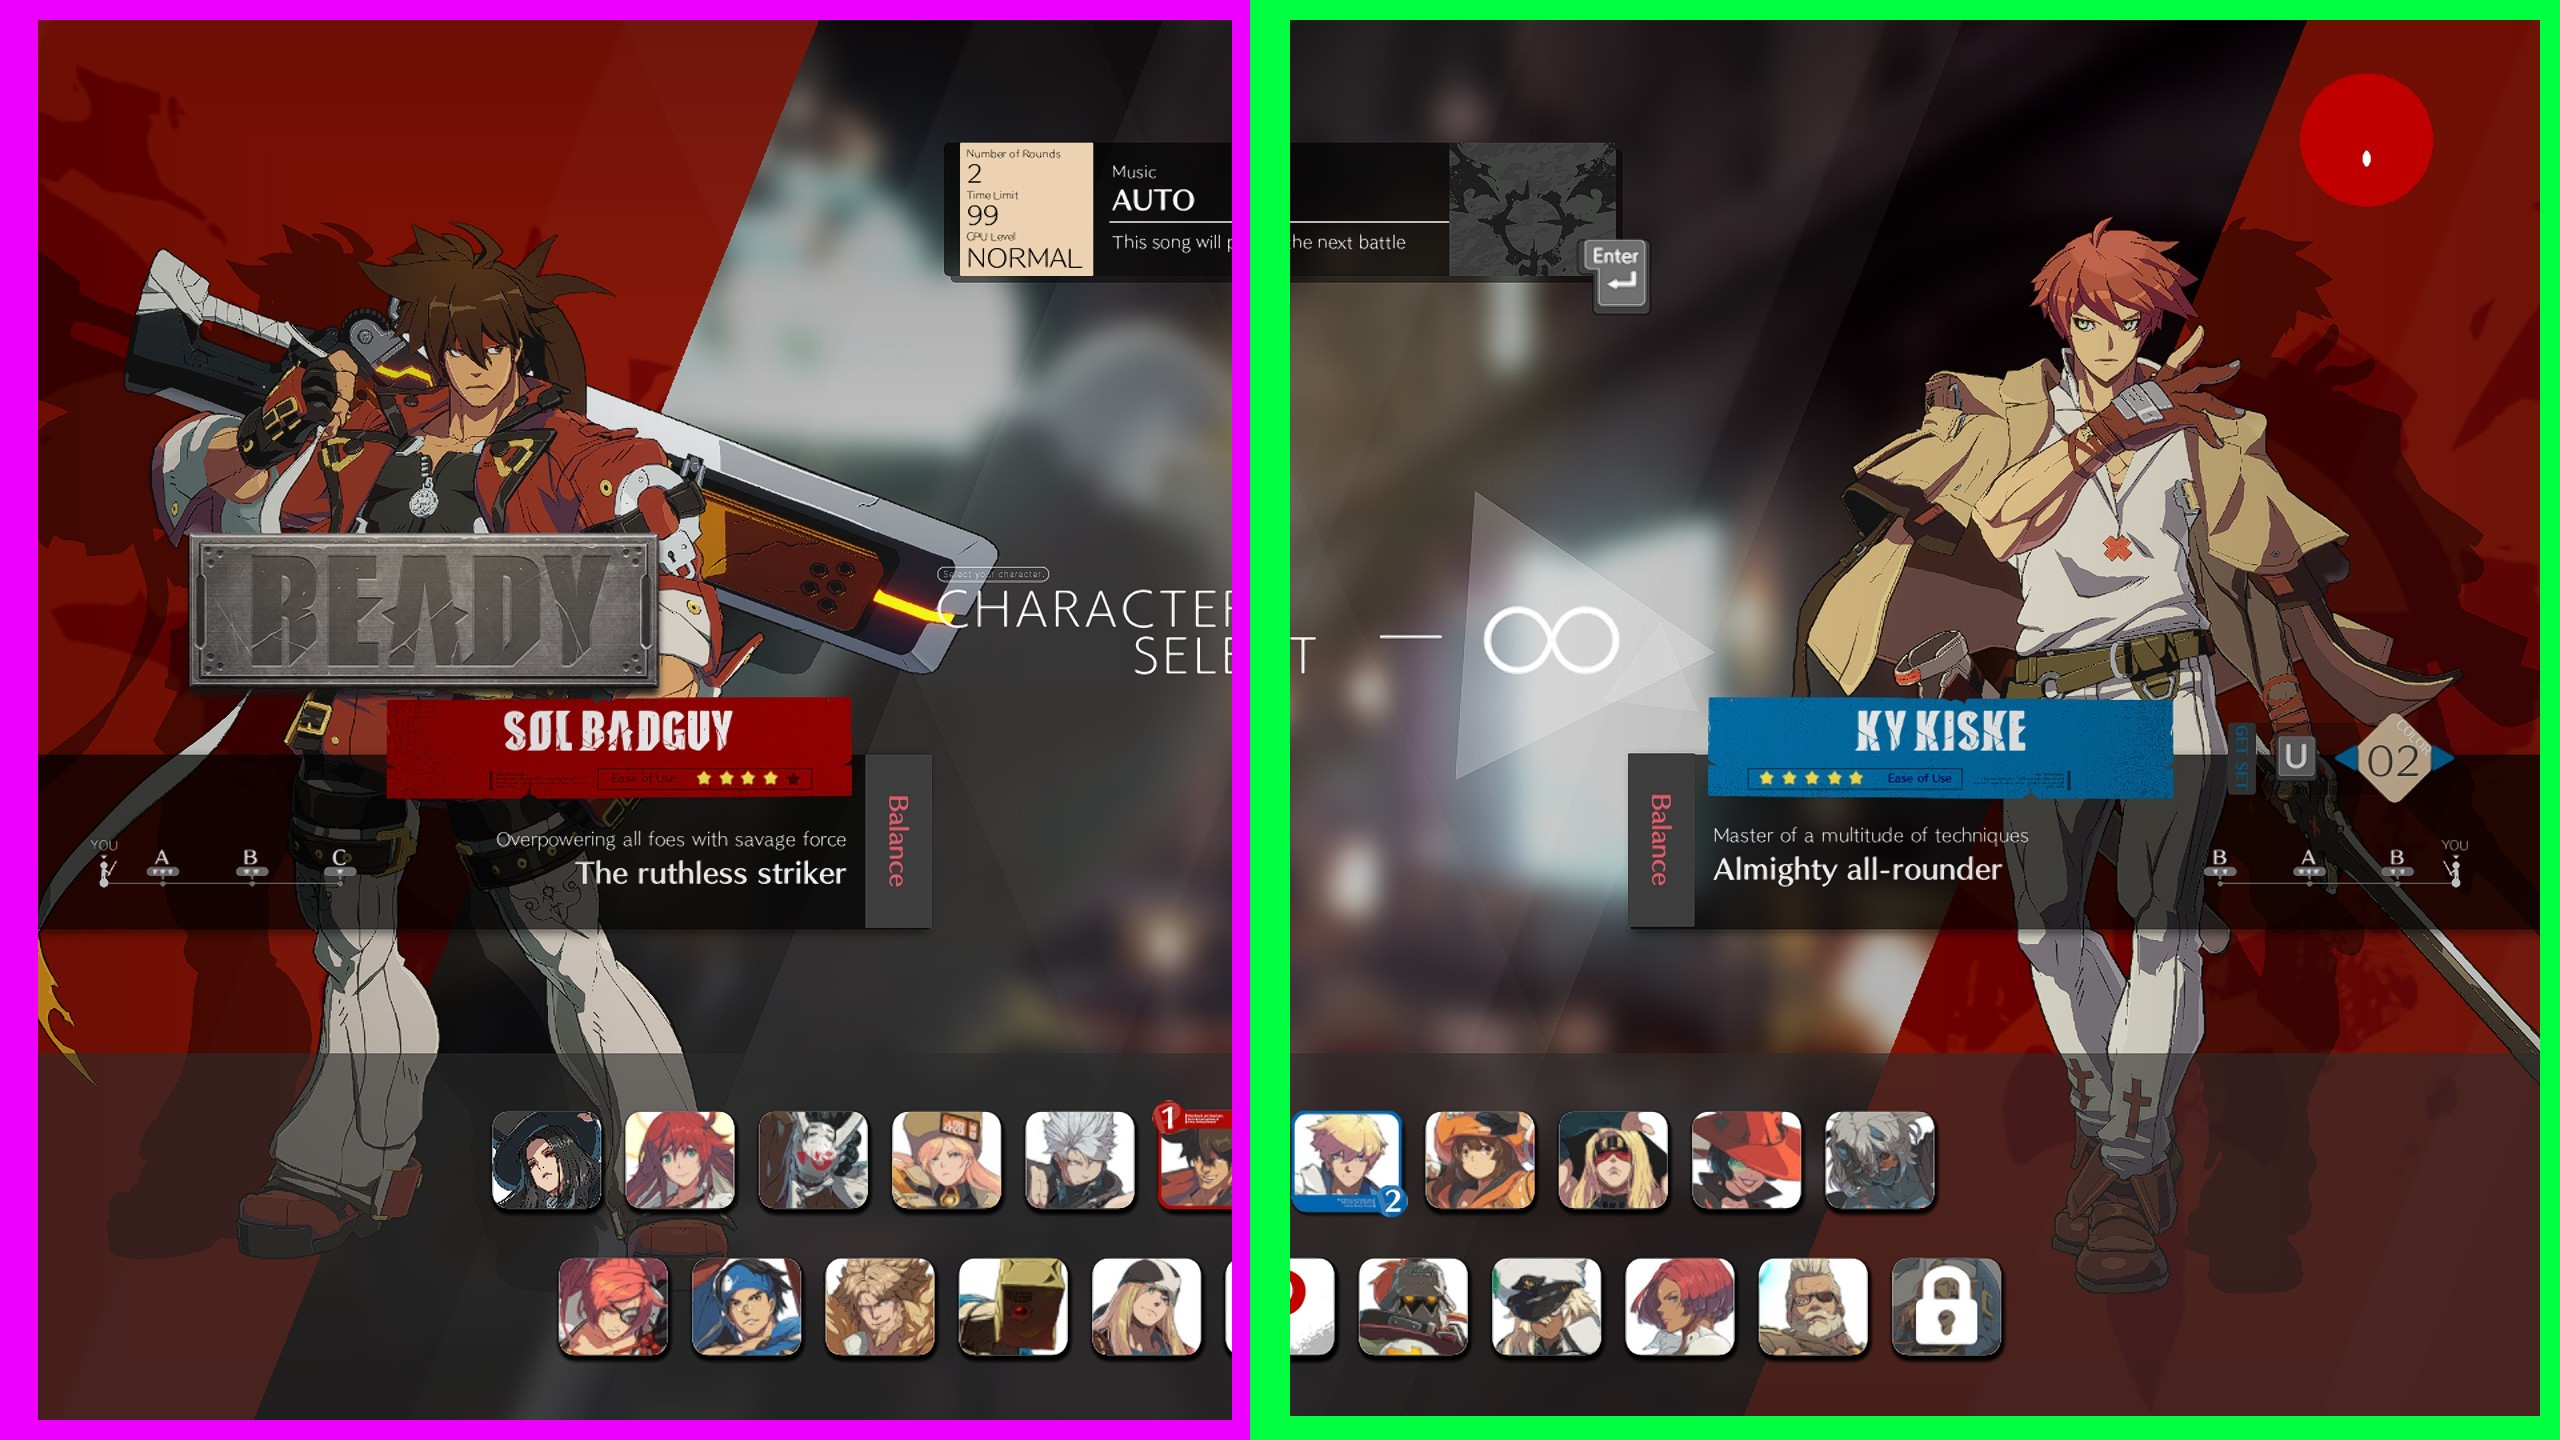
\includegraphics[height=0.5\textwidth]{figures/guilty.jpg}
    \label{fig: strive chracter select}
\end{figure}

Lo mismo ocurre en otros juegos como Melty Blood: Type Lumina \cite{noauthor_melty_nodate}, la figura \ref{fig: melty character select}:

\begin{figure}[ht!]
    \centering
    \caption{Menú de selección de personaje de Melty Blood}
    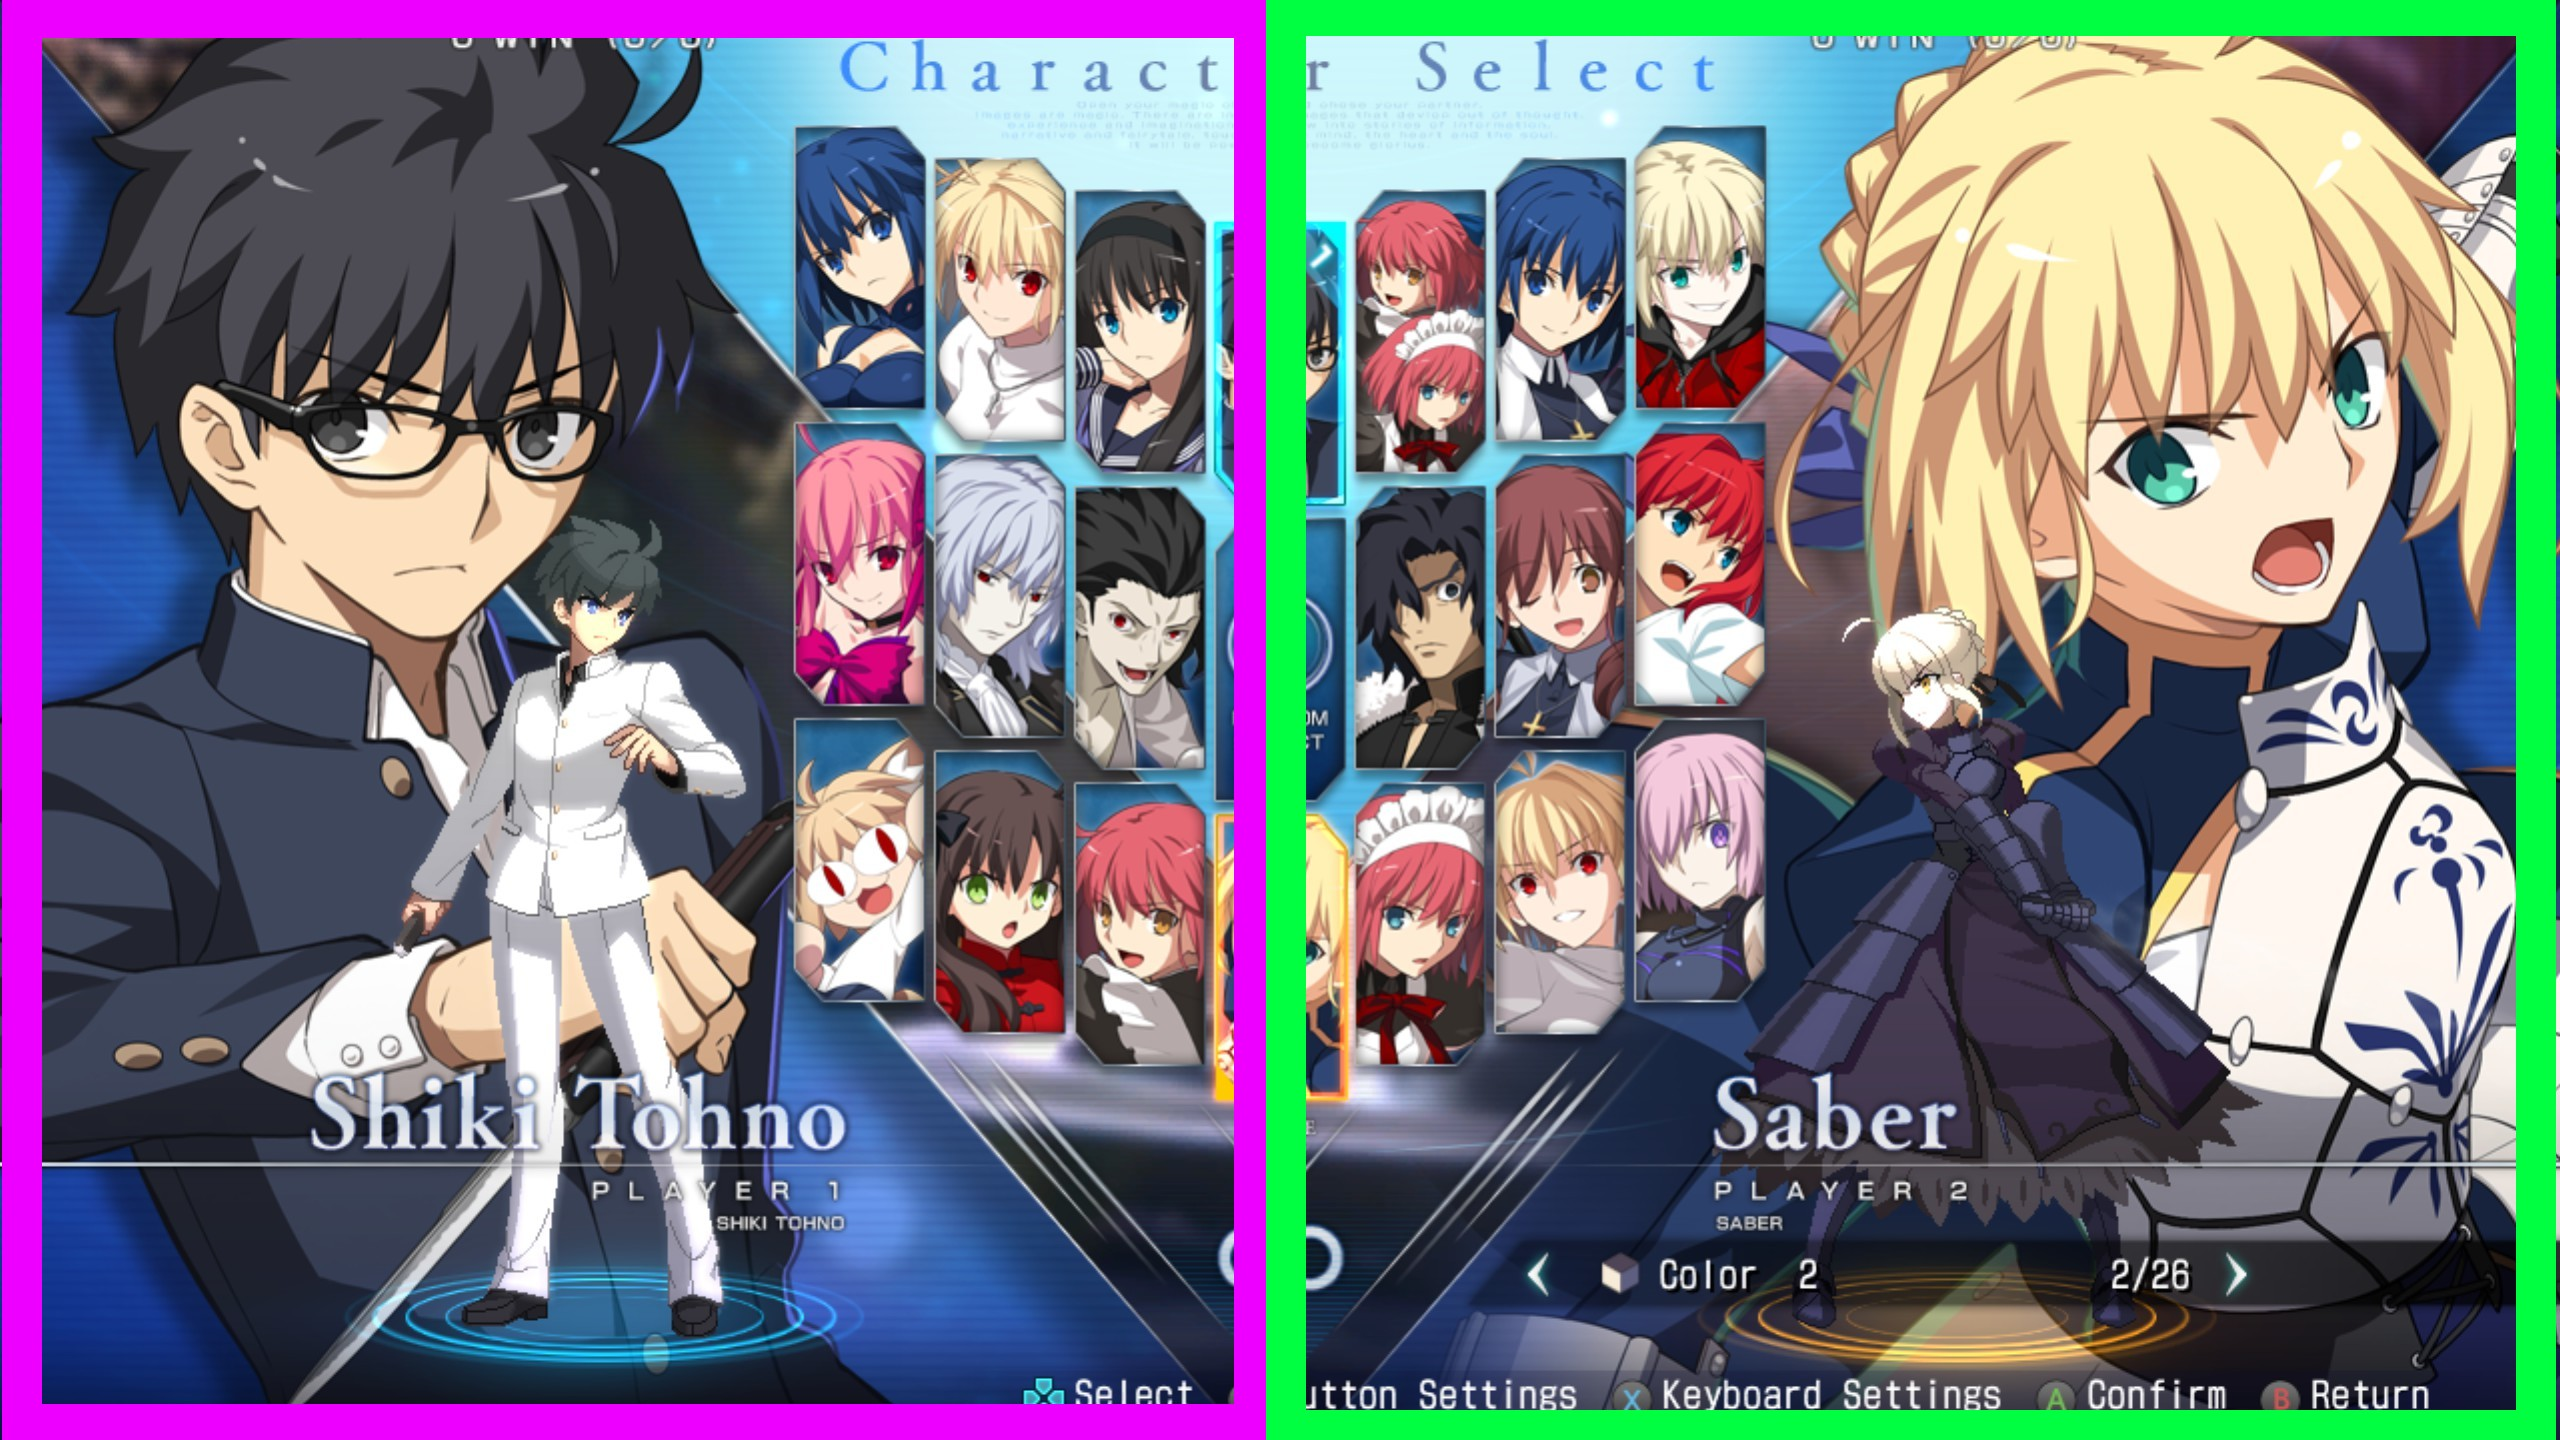
\includegraphics[height=0.5\textwidth]{figures/melty.jpg}
    \label{fig: melty character select}
\end{figure}

Como se ve en ambos ejemplos, los personajes seleccionados están colocados en esquinas opuestas, cada uno en su propia caja. El único elemento que se comparte entre los dos es la lista de personajes (caja azul)

\textbf{Características de la interfaz gráfica}: 

\begin{itemize}
    \item \textbf{Aspectos ergonómicos}
    \begin{itemize}
        \item El texto dentro de la aplicación tiene que ser legible
        \item Los menús desplegables tienen que ser lo suficientemente grande
        \item Se tiene que seguir los estándares de accesibilidad de HTML, tales como el uso de atributos \textit{alt} y el uso apropiado, lógico y consistente de etiquetas
        \item El botón de someter tiene que ser lo suficientemente claro en su propósito y suficientemente grande para que sea cómodo para todo tipo de usuario
    \end{itemize}
    \item \textbf{Colores}
    
    La paleta de colores es la siguiente:
    \begin{figure}[ht!]
        \centering
        \caption{Paleta de Colores}
        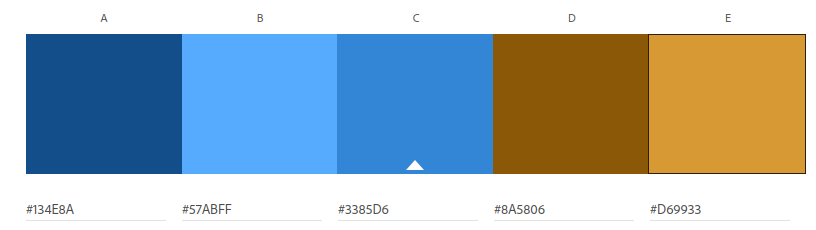
\includegraphics[width=1.0\textwidth]{figures/pallete_updated.png}
        \label{fig: pallete}
    \end{figure}

    Se utiliza el color del medio (\#3385D6 en hexadecimal) como color de fondo. Esto se debe a que al ser azul, distrae al usuario menos que un color como el rojo. Más aún, el color temático de \gls{gbfvs} es el azul claro. Esta relación ayuda a familiarizar el usuario con que juego esta trabajando esta aplicación. El color que se usa para los bordes es el color complementario de \#3385D6, el complemento de \#D69933 (marrón claro). Al marrón ser una mezcla del rojo y el verde, es bueno para detalles y para segmentar elementos de una manera visual.
    \item \textbf{Interactividad}
    \begin{itemize}
        \item Completa
        \begin{itemize}
            \item Imágenes
            \item Apuntador
            \item Teclado
        \end{itemize}
        \item Parcial
        \begin{itemize}
            \item Teclado
            \item Auditivo
        \end{itemize}
    \end{itemize}
    \item \textbf{Validación de datos}
    
    Los fotogramas de cada personaje provienen de \textit{Dustloop} \cite{noauthor_granblue_2022-1}. Estos datos se extraen cada cierto periodo de tiempo de \textit{Dustloop} automáticamente. Se asume que debido a que \gls{gbfvs} ya no está recibiendo actualizaciones que \textit{Dustloop} no cambiará drásticamente la estructura de las páginas de donde se extrae la data. Por ende, se asume que la data fotográmica sera confiable por un buen tiempo.

    Debido a la naturaleza de los menús desplegables, no hay mucha validación necesaria en cuanto a las opciones que se le presentan al usuario. Sin embargo, hay un detalle importante que si se tiene que validar. La aplicación original de \textit{SkyboundDB} tiene la opción de comparar una movida con todas las movidas de otro personaje. Esto implica que no es posible comparar todas las movidas de un personaje con todas de otro por cuestiones de limpieza y por cuestiones prácticas debido a la cantidad de información que se tiene que presentar. A consecuencia de esto, se tiene que validar que el personaje que dio el primer golpe no tenga la opción de \textbf{Seleccionar todas las movidas} seleccionada y que el personaje que responde tampoco lo tenga a la vez. Solo el personaje que responde puede utilizar la opción de seleccionar todas sus movidas. Esta validación se tiene que hacer antes que se haga la comparación.
    % \item \textbf{Consistencia}
    \item \textbf{Carga de memoria}
    
    % Idealmente, la carga de memoria debe ser baja por varias razones: Unas de las metas primordiales de este proyecto es que la aplicación sea rápida y eficiente. Unas de las métricas de eficiencia es la memoria primaria necesaria para mantener la página abierta. Otra métrica importante es la cantidad de banda ancha necesaria para acceder la página en linea. Unos de los casos de usos que tiene la aplicación es su uso en torneos, particularmente entre o antes de partidas. Esta circunstancia requiere que la pagina cargue rápidamente y sin tardarse mucho las comparaciones.  

    En la aplicación original de SkyboundDB, cada personaje tenía su propia foto como ícono para seleccionarlo. Esto hacia que la interfaz sea mas interactiva e intuitiva. Esta decisión era viable porque solo habían 6 personajes, no se añadieron todos los 28 personajes por cuestiones de tiempo. SkyboundDB 2.0 tendrá la opciones se seleccionar cualquier de los 28 personajes. Es por esto que no se puede tener un ícono por cada personaje. Es intimidante tener tanta opciones. Es muy común ver a un jugador novato de juegos de pelea quedarse paralizado al ver cuantos personajes puede usar. Es por esto se tiene que conseguir una manera de colapsar todas las opciones de personajes en un solo elemento, aunque se tenga que sacrificar interactividad.

    \item \textbf{Indicaciones visuales}
    
    Debido a las limitaciones de banda ancha, la página no puede tener una plantilla de estilo demasiada complicada. Sin embargo, elementos sencillos pueden mejorar la experiencia de usuario sin sacrificar mucho en términos de rapidez. Una imagen simple del personaje que se ha seleccionado, como se presenta en la figura \ref{fig: melty character select}, puede ayudar corroborar rápidamente si la selección del usuario fue la que quiso. Además, se puede estilizar la selección de movida para que se asemeje mas a la selección de traje como se puede apreciar con el dígito $2$ con las flechas en la parte derecha de las figuras \ref{fig: strive chracter select} y \ref{fig: melty character select}. Estos detalles ayudan a conformarse al modelo mental que tiene el usuario de los juegos de pelea.
\end{itemize}

\chapter{Aspectos Tecnológicos}
\addcontentsline{toc}{chapter}{Aspectos Tecnológicos}

\begin{table}
    \caption{Aspectos Tecnológicos}
    
\begin{tabularx}{\textwidth}{| X | X | X |}
    \hline
    \textbf{Tipo de dispositivos} & \textbf{Descripción} & \textbf{Ejemplos} \\
    \hline
    \textbf{Entrada} & Los usuarios entran la data mediante un dispositivo apuntador en las cajas de selección multiples las movidas de tanto el personaje que hace la movida y el personaje que recibe la movida & Ratón, teclado y lápiz óptico como medios de entrada. \\
    \hline
    \textbf{Salida} & Se proyecta los resultados de la comparación mediante una pantalla o mediante ayuda de sonido por parte de asistencia de una aplicación lectora. & Monitor, altavoz, bocinas y auriculares como medios de salida. \\
    \hline
    \textbf{Entrada/Salida} & Los usuarios lo usan para tanto entrar la información mediante las cajas de selección multiples y a su vez se le presenta la información de las comparaciones mediante el mismo dispositivo. & Pantalla táctil. (teléfono y tablet). \\
    \hline
\end{tabularx}

\label{tab: aspectos tec}
\end{table}

\textbf{Estilos de Interacción}: Se toma en mente que este programa solo se puede acceder desde el internet, pues es una pagina Web. Bajo esta lógica, se sigue que, por razones de ancho de banda, la pagina no debe tener mucho estilo (como imágenes de todas las movidas e imágenes decorativas) para asi no tomar tiempo cargando dicha pagina y substraendo de su sentido práctico. Por eso la pagina se hace todo dentro de un mismo documento HTML que se alimenta de un CSS y un JS, de manera que en todo momento la información necesaria esta viva y no tiene que cargar nada en adicional. Esto deja que la mayoría del tiempo que un usuario este interactuando con la pagina terminará siendo el tiempo que tomen en escoger los personajes y sus movidas. Esto también se ha facilitado, pues las listas de personajes se organizaron de manera alfabética y esto permite que el usuario pueda navegar por rangos en el teclado presionando la primera letra del nombre del personaje que se esta hallando. 

También se presenta los resultados como listados tabulados con colores para saber qué tipo de movimiento es (si es un botón liviano-rosa, mediano-verde, o pesado-rojo) para dejarle saber al usuario sin necesitar imágenes y de la manera más simple pero organizada los resultados de dicha situación proveída por el usuario.

\textbf{Características de la Interfaz Gráfica de Usuarios}: Las opciones se podrán acceder mediante un dispositivo apuntador que el usuario decida usar. Esto entonces nos deja con que el usuario nominalmente puede usar cualquier dispositivo que tenga capacidad de usar un navegador web y algún tipo de dispositivo apuntador para interactuar con ella, sea un lápiz óptico en una tablet o (el comúnmente usado) ratón. Cómo manera adicional de acceder la aplicación en la web, los usuarios pueden someter la información atravéz de una pantalla táctil que funciona tanto como un dispositivo de entrada para la información, asi como la salida (se presenta los resultados en la misma pantalla). Consecuentemente, al ser una aplicación web, no habrá muchas otras maneras de interactuar con ella más que con las cajas de selección y por aplicaciones de texto a altavoz mediante los textos alternativos proveídos para justamente esa necesidad (de faltar ayuda auditoria en vez de visión).

\printglossary[type=\acronymtype]

\bibliography{References}

\bibliographystyle{apacite}

\end{document}
